% Options for packages loaded elsewhere
\PassOptionsToPackage{unicode}{hyperref}
\PassOptionsToPackage{hyphens}{url}
%
\documentclass[
]{article}
\usepackage{amsmath,amssymb}
\usepackage{lmodern}
\usepackage{ifxetex,ifluatex}
\ifnum 0\ifxetex 1\fi\ifluatex 1\fi=0 % if pdftex
  \usepackage[T1]{fontenc}
  \usepackage[utf8]{inputenc}
  \usepackage{textcomp} % provide euro and other symbols
\else % if luatex or xetex
  \usepackage{unicode-math}
  \defaultfontfeatures{Scale=MatchLowercase}
  \defaultfontfeatures[\rmfamily]{Ligatures=TeX,Scale=1}
\fi
% Use upquote if available, for straight quotes in verbatim environments
\IfFileExists{upquote.sty}{\usepackage{upquote}}{}
\IfFileExists{microtype.sty}{% use microtype if available
  \usepackage[]{microtype}
  \UseMicrotypeSet[protrusion]{basicmath} % disable protrusion for tt fonts
}{}
\makeatletter
\@ifundefined{KOMAClassName}{% if non-KOMA class
  \IfFileExists{parskip.sty}{%
    \usepackage{parskip}
  }{% else
    \setlength{\parindent}{0pt}
    \setlength{\parskip}{6pt plus 2pt minus 1pt}}
}{% if KOMA class
  \KOMAoptions{parskip=half}}
\makeatother
\usepackage{xcolor}
\IfFileExists{xurl.sty}{\usepackage{xurl}}{} % add URL line breaks if available
\IfFileExists{bookmark.sty}{\usepackage{bookmark}}{\usepackage{hyperref}}
\hypersetup{
  pdftitle={UNILA/BIO0039 - Exercício prático aula 14},
  pdfauthor={Peter Löwenberg Neto},
  hidelinks,
  pdfcreator={LaTeX via pandoc}}
\urlstyle{same} % disable monospaced font for URLs
\usepackage[margin=1in]{geometry}
\usepackage{color}
\usepackage{fancyvrb}
\newcommand{\VerbBar}{|}
\newcommand{\VERB}{\Verb[commandchars=\\\{\}]}
\DefineVerbatimEnvironment{Highlighting}{Verbatim}{commandchars=\\\{\}}
% Add ',fontsize=\small' for more characters per line
\usepackage{framed}
\definecolor{shadecolor}{RGB}{248,248,248}
\newenvironment{Shaded}{\begin{snugshade}}{\end{snugshade}}
\newcommand{\AlertTok}[1]{\textcolor[rgb]{0.94,0.16,0.16}{#1}}
\newcommand{\AnnotationTok}[1]{\textcolor[rgb]{0.56,0.35,0.01}{\textbf{\textit{#1}}}}
\newcommand{\AttributeTok}[1]{\textcolor[rgb]{0.77,0.63,0.00}{#1}}
\newcommand{\BaseNTok}[1]{\textcolor[rgb]{0.00,0.00,0.81}{#1}}
\newcommand{\BuiltInTok}[1]{#1}
\newcommand{\CharTok}[1]{\textcolor[rgb]{0.31,0.60,0.02}{#1}}
\newcommand{\CommentTok}[1]{\textcolor[rgb]{0.56,0.35,0.01}{\textit{#1}}}
\newcommand{\CommentVarTok}[1]{\textcolor[rgb]{0.56,0.35,0.01}{\textbf{\textit{#1}}}}
\newcommand{\ConstantTok}[1]{\textcolor[rgb]{0.00,0.00,0.00}{#1}}
\newcommand{\ControlFlowTok}[1]{\textcolor[rgb]{0.13,0.29,0.53}{\textbf{#1}}}
\newcommand{\DataTypeTok}[1]{\textcolor[rgb]{0.13,0.29,0.53}{#1}}
\newcommand{\DecValTok}[1]{\textcolor[rgb]{0.00,0.00,0.81}{#1}}
\newcommand{\DocumentationTok}[1]{\textcolor[rgb]{0.56,0.35,0.01}{\textbf{\textit{#1}}}}
\newcommand{\ErrorTok}[1]{\textcolor[rgb]{0.64,0.00,0.00}{\textbf{#1}}}
\newcommand{\ExtensionTok}[1]{#1}
\newcommand{\FloatTok}[1]{\textcolor[rgb]{0.00,0.00,0.81}{#1}}
\newcommand{\FunctionTok}[1]{\textcolor[rgb]{0.00,0.00,0.00}{#1}}
\newcommand{\ImportTok}[1]{#1}
\newcommand{\InformationTok}[1]{\textcolor[rgb]{0.56,0.35,0.01}{\textbf{\textit{#1}}}}
\newcommand{\KeywordTok}[1]{\textcolor[rgb]{0.13,0.29,0.53}{\textbf{#1}}}
\newcommand{\NormalTok}[1]{#1}
\newcommand{\OperatorTok}[1]{\textcolor[rgb]{0.81,0.36,0.00}{\textbf{#1}}}
\newcommand{\OtherTok}[1]{\textcolor[rgb]{0.56,0.35,0.01}{#1}}
\newcommand{\PreprocessorTok}[1]{\textcolor[rgb]{0.56,0.35,0.01}{\textit{#1}}}
\newcommand{\RegionMarkerTok}[1]{#1}
\newcommand{\SpecialCharTok}[1]{\textcolor[rgb]{0.00,0.00,0.00}{#1}}
\newcommand{\SpecialStringTok}[1]{\textcolor[rgb]{0.31,0.60,0.02}{#1}}
\newcommand{\StringTok}[1]{\textcolor[rgb]{0.31,0.60,0.02}{#1}}
\newcommand{\VariableTok}[1]{\textcolor[rgb]{0.00,0.00,0.00}{#1}}
\newcommand{\VerbatimStringTok}[1]{\textcolor[rgb]{0.31,0.60,0.02}{#1}}
\newcommand{\WarningTok}[1]{\textcolor[rgb]{0.56,0.35,0.01}{\textbf{\textit{#1}}}}
\usepackage{graphicx}
\makeatletter
\def\maxwidth{\ifdim\Gin@nat@width>\linewidth\linewidth\else\Gin@nat@width\fi}
\def\maxheight{\ifdim\Gin@nat@height>\textheight\textheight\else\Gin@nat@height\fi}
\makeatother
% Scale images if necessary, so that they will not overflow the page
% margins by default, and it is still possible to overwrite the defaults
% using explicit options in \includegraphics[width, height, ...]{}
\setkeys{Gin}{width=\maxwidth,height=\maxheight,keepaspectratio}
% Set default figure placement to htbp
\makeatletter
\def\fps@figure{htbp}
\makeatother
\setlength{\emergencystretch}{3em} % prevent overfull lines
\providecommand{\tightlist}{%
  \setlength{\itemsep}{0pt}\setlength{\parskip}{0pt}}
\setcounter{secnumdepth}{-\maxdimen} % remove section numbering
\ifluatex
  \usepackage{selnolig}  % disable illegal ligatures
\fi

\title{UNILA/BIO0039 - Exercício prático aula 14}
\author{Peter Löwenberg Neto}
\date{17/09/2021}

\begin{document}
\maketitle

\hypertarget{objetivo-do-exercuxedcio}{%
\subsubsection{1. Objetivo do
exercício}\label{objetivo-do-exercuxedcio}}

Neste exercício você irá abrir e plotar uma filogenia. Depois irá obter
o número de linhagens ao longo do tempo. Para realizar este exercício
você deverá instalr o programa R e o programa RStudio em seu computador.

\hypertarget{instalauxe7uxe3o}{%
\subsubsection{2. Instalação}\label{instalauxe7uxe3o}}

Instalar o R (\url{https://www.r-project.org/}).

Instalar o RStudio
(\url{https://www.rstudio.com/products/rstudio/download/}).

\hypertarget{instalar-o-pacote-no-r}{%
\paragraph{2.1 Instalar o pacote no R}\label{instalar-o-pacote-no-r}}

Executar o RStudio e na linha de comando instalar o pacote

\begin{Shaded}
\begin{Highlighting}[]
\FunctionTok{install.packages}\NormalTok{(}\StringTok{\textquotesingle{}ape\textquotesingle{}}\NormalTok{)}
\end{Highlighting}
\end{Shaded}

\hypertarget{carregar-o-pacote-ape}{%
\subsubsection{3. Carregar o pacote ape}\label{carregar-o-pacote-ape}}

\begin{Shaded}
\begin{Highlighting}[]
\FunctionTok{library}\NormalTok{(ape)}
\end{Highlighting}
\end{Shaded}

\hypertarget{determinar-a-pasta-de-trabalho-arquivo-onde-estuxe3o-os-dados}{%
\subsubsection{4. Determinar a pasta de trabalho (arquivo onde estão os
dados)}\label{determinar-a-pasta-de-trabalho-arquivo-onde-estuxe3o-os-dados}}

Aqui você deve mudar o endereço para a sua pasta.\\
Nesta pasta você irá salvar o arquivo platytree.newick que está no
Moodle.

\begin{Shaded}
\begin{Highlighting}[]
\FunctionTok{setwd}\NormalTok{(}\StringTok{"D:/Usuários/peter/OneDrive/R/LTT"}\NormalTok{)}
\end{Highlighting}
\end{Shaded}

\hypertarget{carregar-a-uxe1rvore-filogenuxe9tica-do-arquivo}{%
\subsubsection{5. Carregar a árvore filogenética do
arquivo}\label{carregar-a-uxe1rvore-filogenuxe9tica-do-arquivo}}

Vamos criar um objeto (af) que conterá nossa árvore filogenética.

\begin{Shaded}
\begin{Highlighting}[]
\NormalTok{af }\OtherTok{\textless{}{-}} \FunctionTok{read.tree}\NormalTok{(}\AttributeTok{file =} \StringTok{"platytree.newick"}\NormalTok{)}
\NormalTok{af}
\end{Highlighting}
\end{Shaded}

\begin{verbatim}
## 
## Phylogenetic tree with 84 tips and 83 internal nodes.
## 
## Tip labels:
##   Cacajao_calvus, Cacajao_hosomi, Chiropotes_chiropotes, Chiropotes_utahickae, Pithecia_pithecia, Pithecia_monachus, ...
## 
## Rooted; includes branch lengths.
\end{verbatim}

\hypertarget{plotar-a-uxe1rvore-filogenuxe9tica}{%
\subsubsection{6. Plotar a árvore
filogenética}\label{plotar-a-uxe1rvore-filogenuxe9tica}}

Observe que a árvore apresenta os comprimentos de ramos proporcionais ao
tempo. Ou seja, é uma filogenia com calibração temporal (= cronograma).

\begin{Shaded}
\begin{Highlighting}[]
\FunctionTok{plot}\NormalTok{(af, }\AttributeTok{cex =} \FloatTok{0.5}\NormalTok{)}
\end{Highlighting}
\end{Shaded}

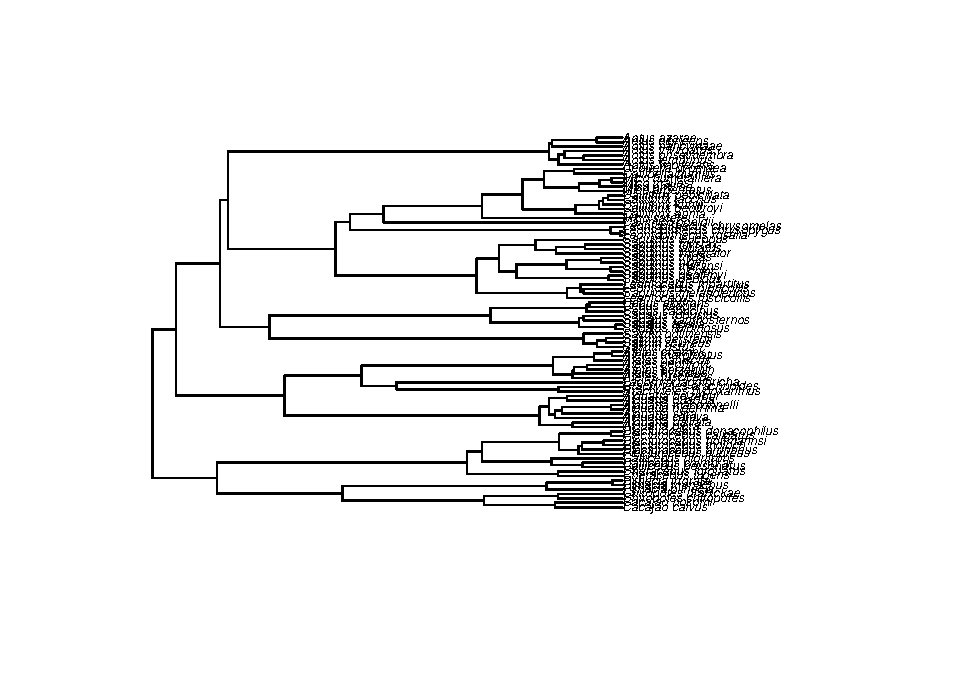
\includegraphics{ex14_files/figure-latex/unnamed-chunk-5-1.pdf}

\hypertarget{obter-o-nuxfamero-de-linhagens-ao-longo-do-tempo.}{%
\subsubsection{7. Obter o número de linhagens ao longo do
tempo.}\label{obter-o-nuxfamero-de-linhagens-ao-longo-do-tempo.}}

Observe o número de linhagens existentes ao longo do tempo.\\
O eixo x representa o tempo e o eixo y representa o número de linhagens.

\begin{Shaded}
\begin{Highlighting}[]
\FunctionTok{ltt.plot}\NormalTok{(af)}
\end{Highlighting}
\end{Shaded}

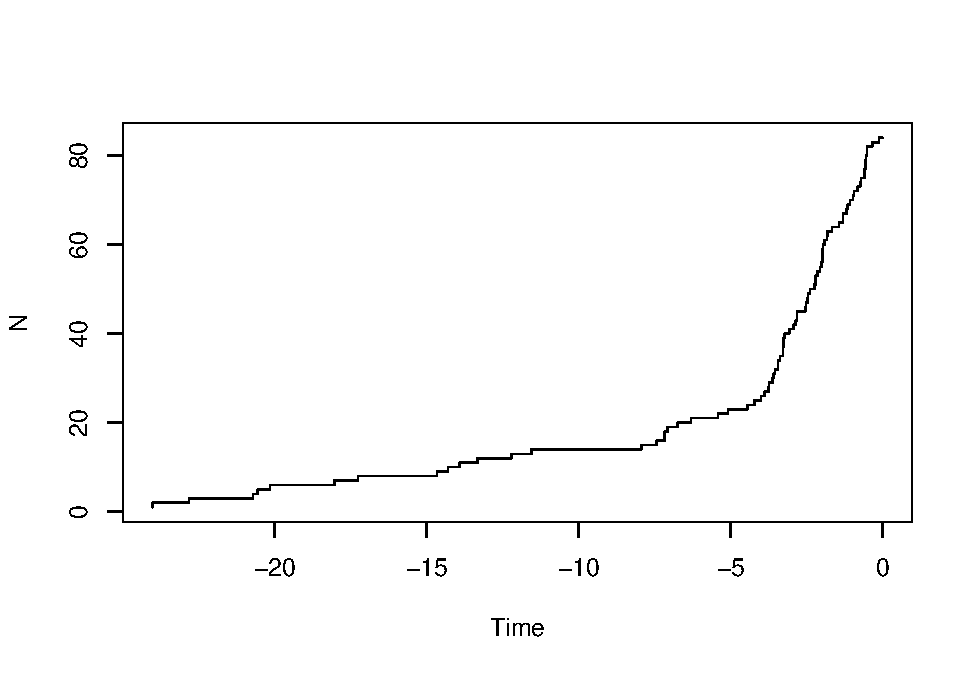
\includegraphics{ex14_files/figure-latex/unnamed-chunk-6-1.pdf}

\hypertarget{salvar-figura-de-linhagens-ao-longo-do-tempo-e-enviar-via-moodle.}{%
\subsubsection{8. Salvar figura de linhagens ao longo do tempo e enviar
via
Moodle.}\label{salvar-figura-de-linhagens-ao-longo-do-tempo-e-enviar-via-moodle.}}

\end{document}
